\documentclass[journal]{IEEEtran}

% *** CITATION PACKAGES ***
\usepackage[style=ieee]{biblatex} 
\bibliography{analog.bib}    %your file created using JabRef
\usepackage{hyperref}
% *** MATH PACKAGES ***
\usepackage{amsmath}
 \usepackage{multirow}

% *** PDF, URL AND HYPERLINK PACKAGES ***
\usepackage{url}
% correct bad hyphenation here
\hyphenation{op-tical net-works semi-conduc-tor}
\usepackage{graphicx}  %needed to include png, eps figures
\usepackage{float}  % used to fix location of images i.e.\begin{figure}[H]

\begin{document}

% paper title
\title{Laboratorio di elettronica analogica\\ 
%\small{1 gennaio 2020}
}

% author names 
\author{\begin{center}Matteo Barbagiovanni\textsuperscript{1},
        Stefano Barbero\textsuperscript{2},
        Federico Malnati\textsuperscript{3},
        Valerio Pagliarino\textsuperscript{4},
        {\small \\
        \textsuperscript{1}
        matteo.barbagiovanni@edu.unito.it -
        \textsuperscript{2}
        stefano.barbero376@edu.unito.it
        \textsuperscript{3}
        federico.malnati@edu.unito.it -
        \textsuperscript{4}
        valerio.pagliarino@edu.unito.it}
        \end{center}}% <-this % stops a space
        
% The report headers
\markboth{Universita' degli Studi di Torino - C.d.L. Triennale in Fisica - 01/01/19 - A.A. 2021-2022    \quad   \quad \quad \quad   \quad \quad \quad  \quad   \quad \quad \quad   \quad \quad LABORATORIO DI ELETTRONICA \quad \quad }%do not delete next lines
{Shell \MakeLowercase{\textit{et al.}}: Bare Demo of IEEEtran.cls for IEEE Journals}

% make the title area
\maketitle

% As a general rule, do not put math, special symbols or citations
% in the abstract or keywords.
\begin{abstract}  
Due righe di introduzione: focus della relazione sull'elettronica analogica, sua importanza per la costruzione di apparati, rivelatori e nella ricerca in fisica. Focus su elementi attivi di base a semiconduttore (diodo), prosecuzione con caratterizzazione degli OpAmp e circuiti notevoli che si possono realizzare grazie a loro, conclusione con elementi di optoelettronica: LED, SiPM. Linee di tramissione.
\end{abstract}


%%%%%%%%%%%%%%%%%%%%%%%%%%%%%%%%%%%%%%%%%%
\section{Strumentazione utilizzata} %Valerio

\IEEEPARstart{D}{escrizione:} della strumentazione utilizzata in laboratorio generica (elenco... abbiamo lavorato su breadbord).

\subsection{\textbf{Oscilloscopio Tektronix}}
Descrizione specifiche tecniche del device e suo utilizzo e sue peculiarità. [DSO = Digital storage oscilloscope]

\subsection{\textbf{Oscilloscopio Rhode & Schwartz}}
Descrizione specifiche tecniche 
Descrizione specifiche tecniche del device e suo utilizzo e sue peculiarità (banda 70 MHz, ma 2.5 GSa/s acquisizione!)
[DPO = Digital phosphore oscilloscope]

\subsection{\textbf{Generatore di funzioni Rigol DG1022Z}}
Descrizione

\subsection{\textbf{Generatore di impulsi veloci Keythley ...}}
Descrizione

\subsection{\textbf{Multimetro digitale}}
Descrizione

\subsection{\textbf{Alimentatore da banco DUALE GW-Instek}}
Descrizione

%%%%%%%%%%%%%%%%%%%%%%%%%%%%%%%%%%%%%%%%%%
\section{\textbf{Ponte raddrizzatore a diodi a singola semionda}} %Matteo
introduzione funzionamento 
risposta ottenuta in linea con quella attesa
DV controllo con materiale

\begin{figure}[H]%[!ht]
\begin {center}
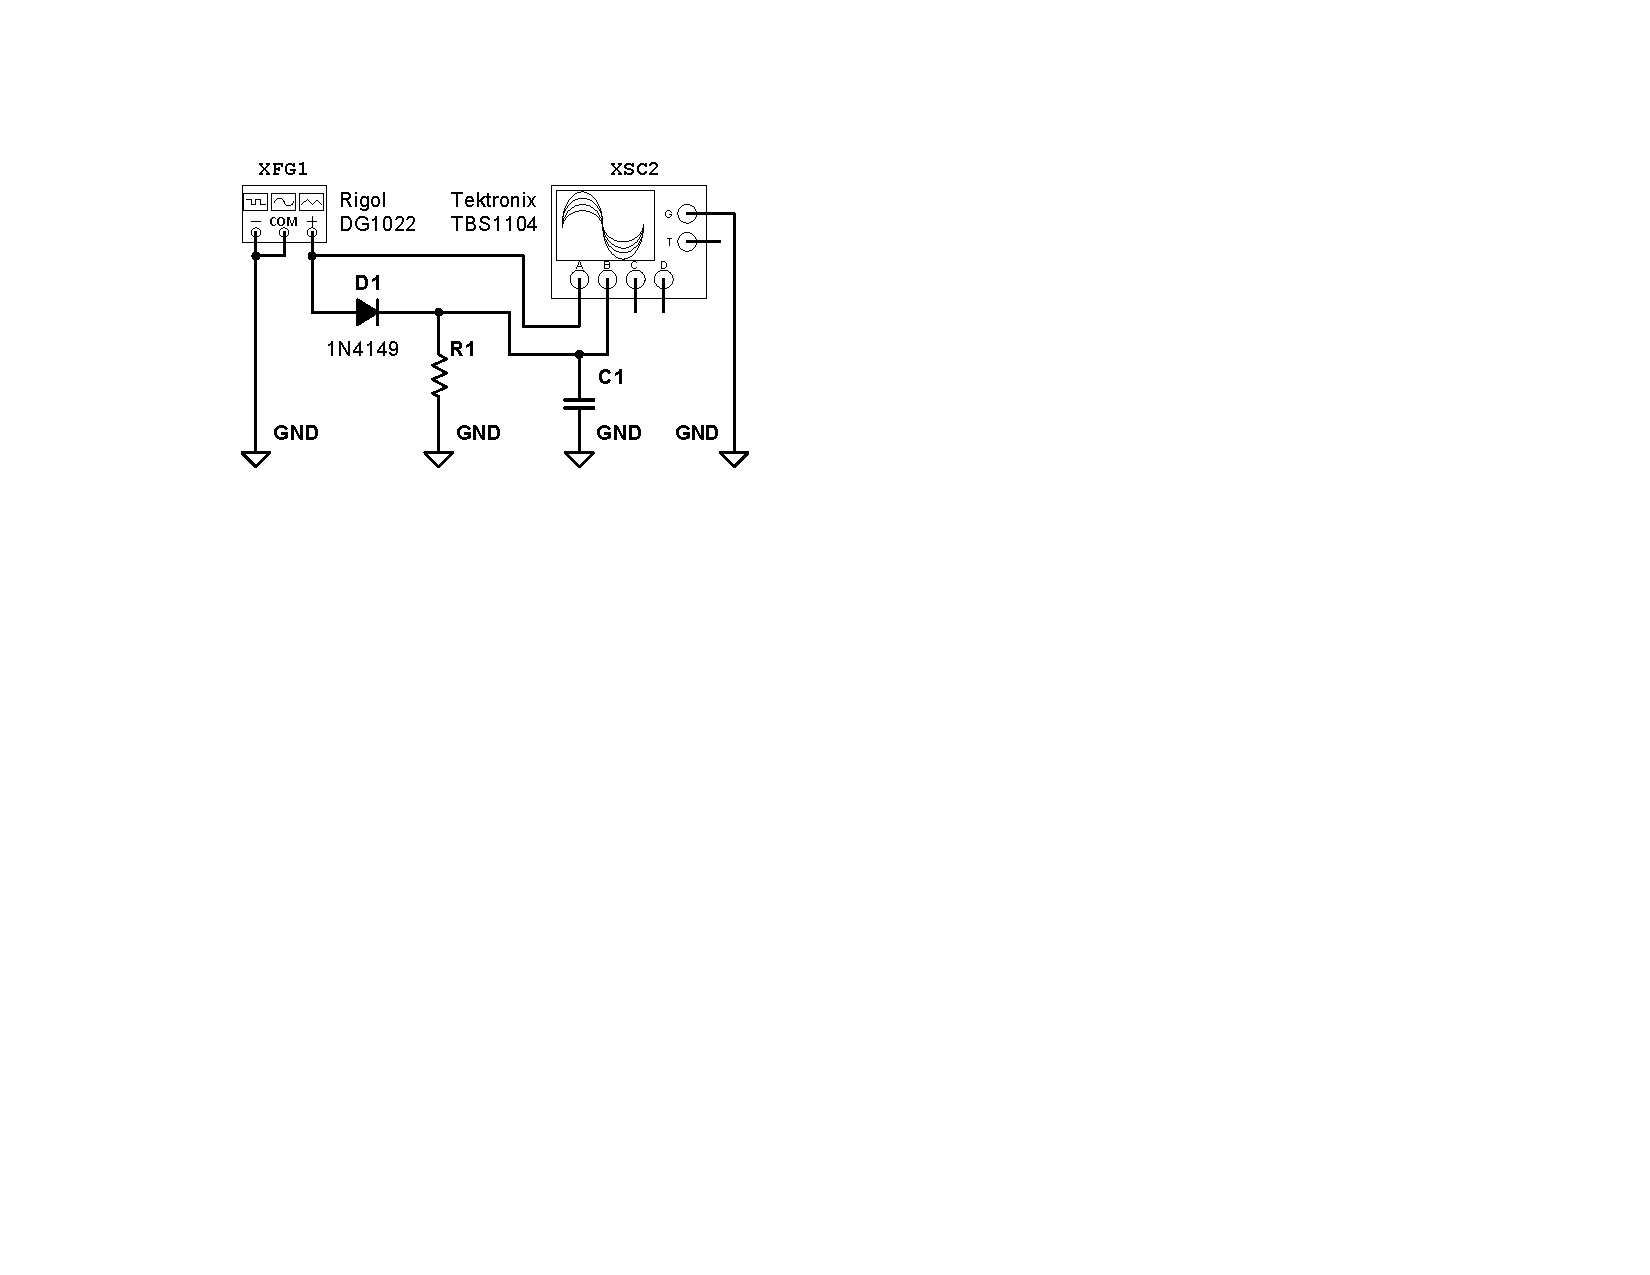
\includegraphics[width=0.38\textwidth]{sch-simulations/output/Diode-rectifier.pdf}
\caption{Didascalia}
\label{fig:oscilloscope}
\end {center}
\end{figure}

\subsection{\textbf{Introduzione all'esperienza}}
Descrizione

\subsection{\textbf{Componentistica e circuito}}
Descrizione

\subsection{\textbf{Caratterizzazione}}
Descrizione

\subsection{\textbf{Discussione dei risultati}}
Descrizione


%%%%%%%%%%%%%%%%%%%%%%%%%%%%%%%%%%%%%%%%%%
\section{\textbf{Introduzione all'amplificatore operazionale}}
Descrizione generale dell'OPA %Valerio

\subsection{\textbf{Integrato LM741}}
Descrizione specifica dal datasheet


%%%%%%%%%%%%%%%%%%%%%%%%%%%%%%%%%%%%%%%%%%
\section{\textbf{Anello aperto invertente (zero-crossing detector)}} %Stefano
Descrizione

\begin{figure}[H]%[!ht]
\begin {center}
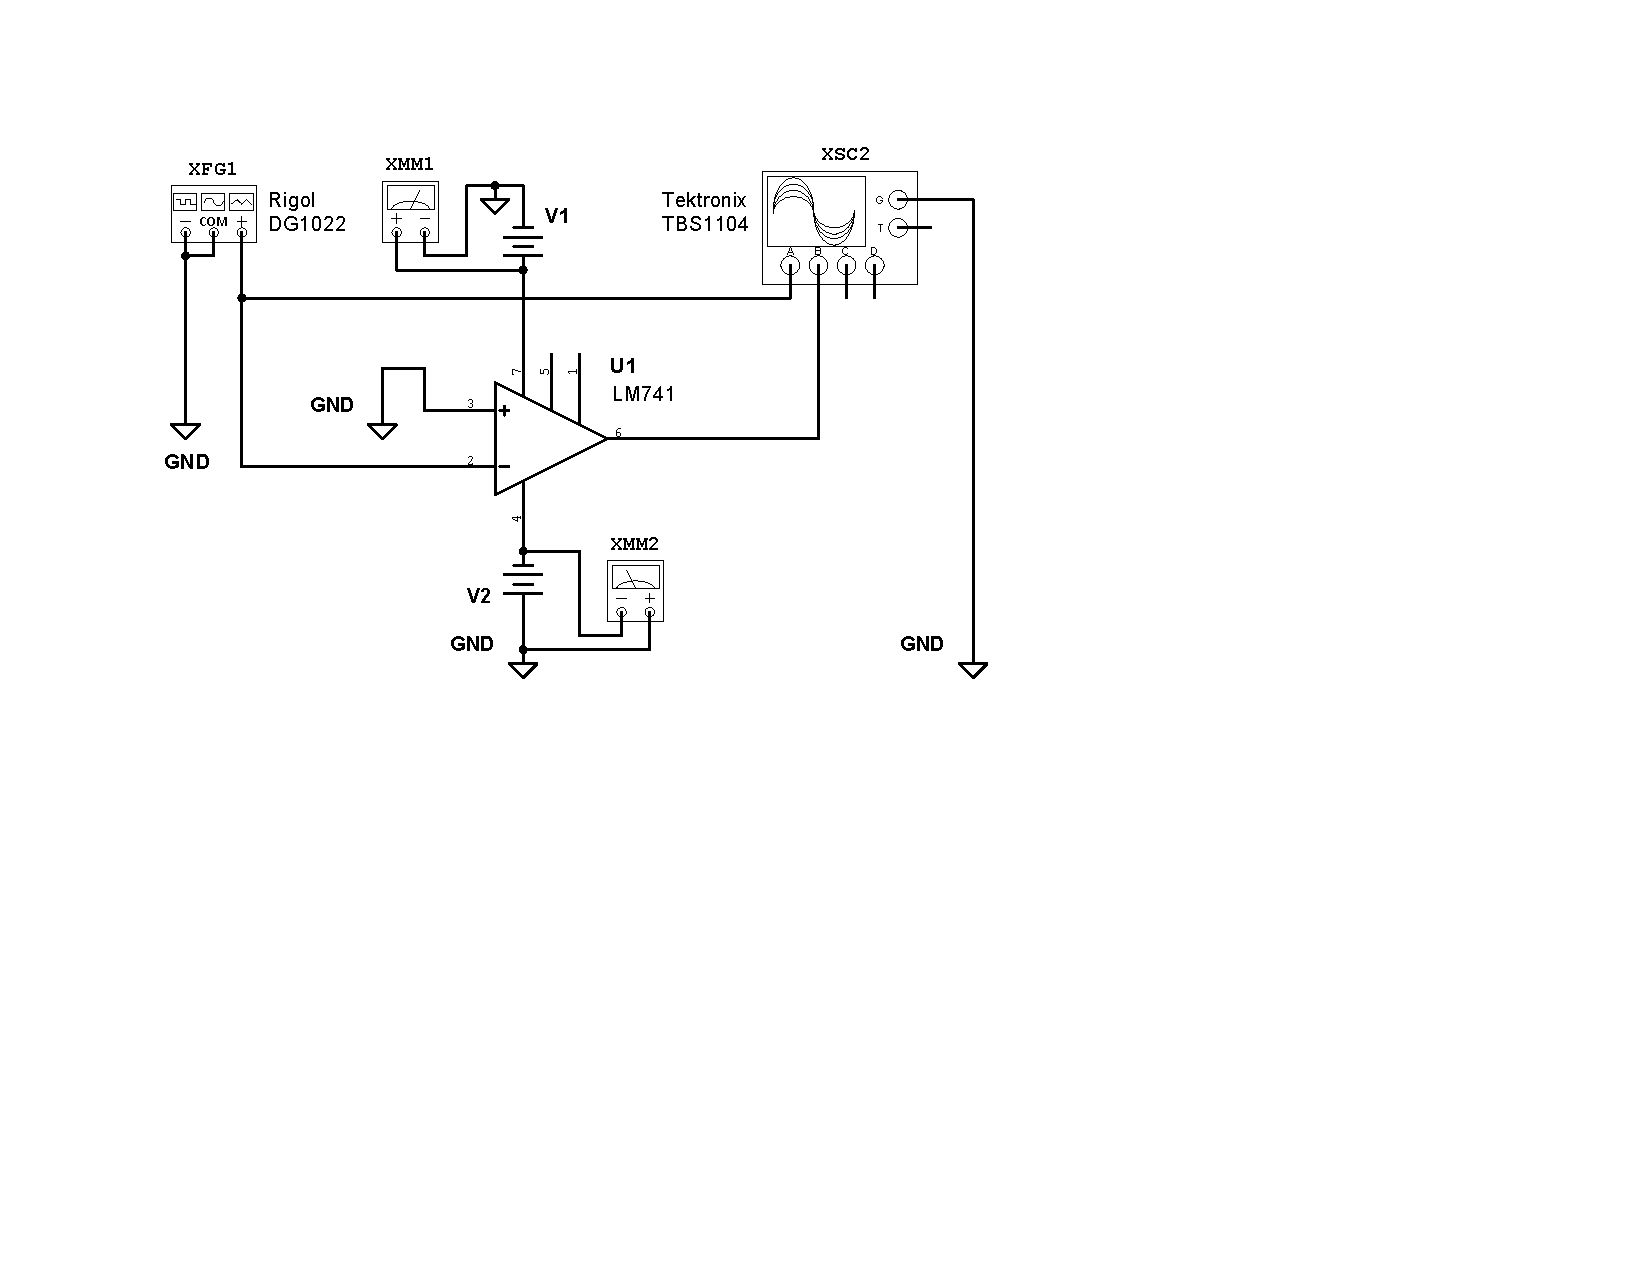
\includegraphics[width=0.38\textwidth]{sch-simulations/output/OPA-open-loop-inverting.pdf}
\caption{Didascalia}
\label{fig:oscilloscope}
\end {center}
\end{figure}


%%%%%%%%%%%%%%%%%%%%%%%%%%%%%%%%%%%%%%%%%%
\section{\textbf{Anello aperto non invertente}} %Stefano
Descrizione

\begin{figure}[H]%[!ht]
\begin {center}
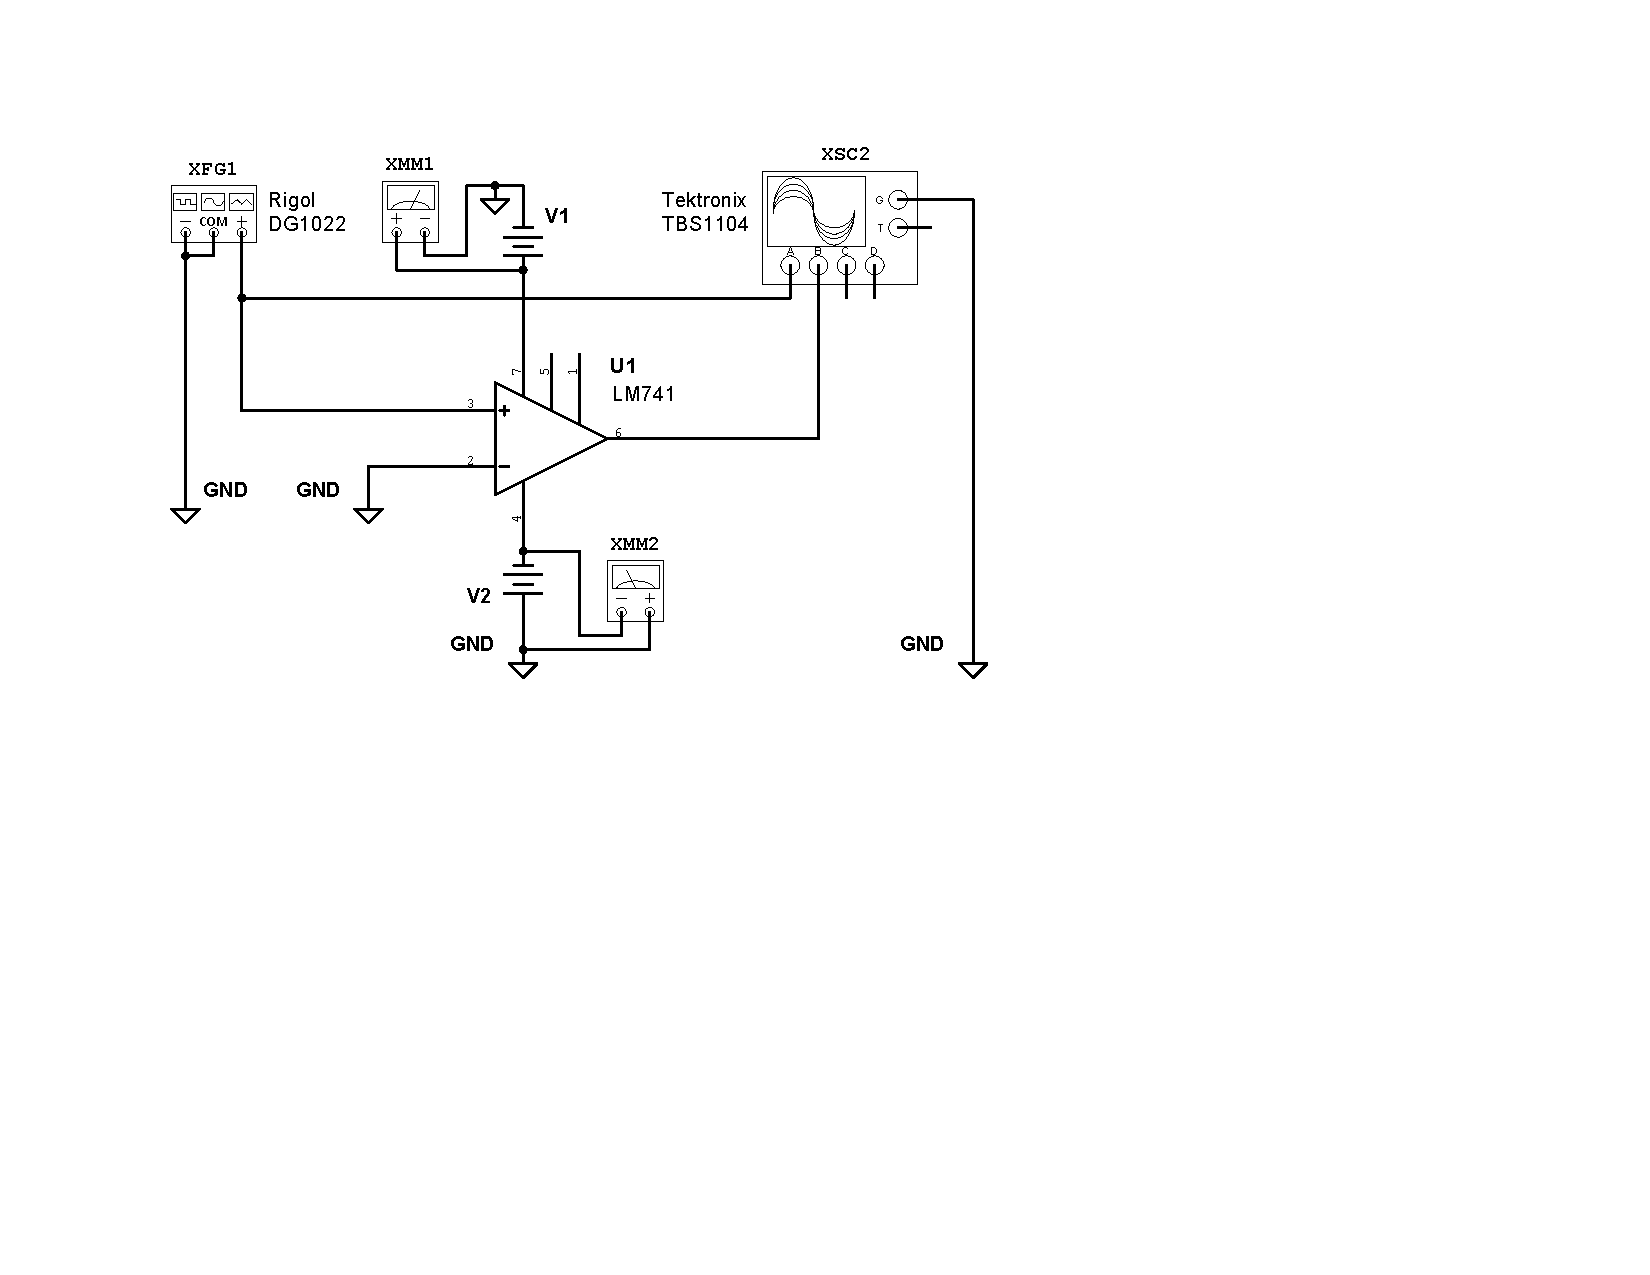
\includegraphics[width=0.38\textwidth]{sch-simulations/output/OPA-open-loop-non-inverting.pdf}
\caption{Didascalia}
\label{fig:oscilloscope}
\end {center}
\end{figure}


%%%%%%%%%%%%%%%%%%%%%%%%%%%%%%%%%%%%%%%%%%
\section{\textbf{Amplificatore reazionato invertente}} %Stefano
Descrizione

\begin{figure}[H]%[!ht]
\begin {center}
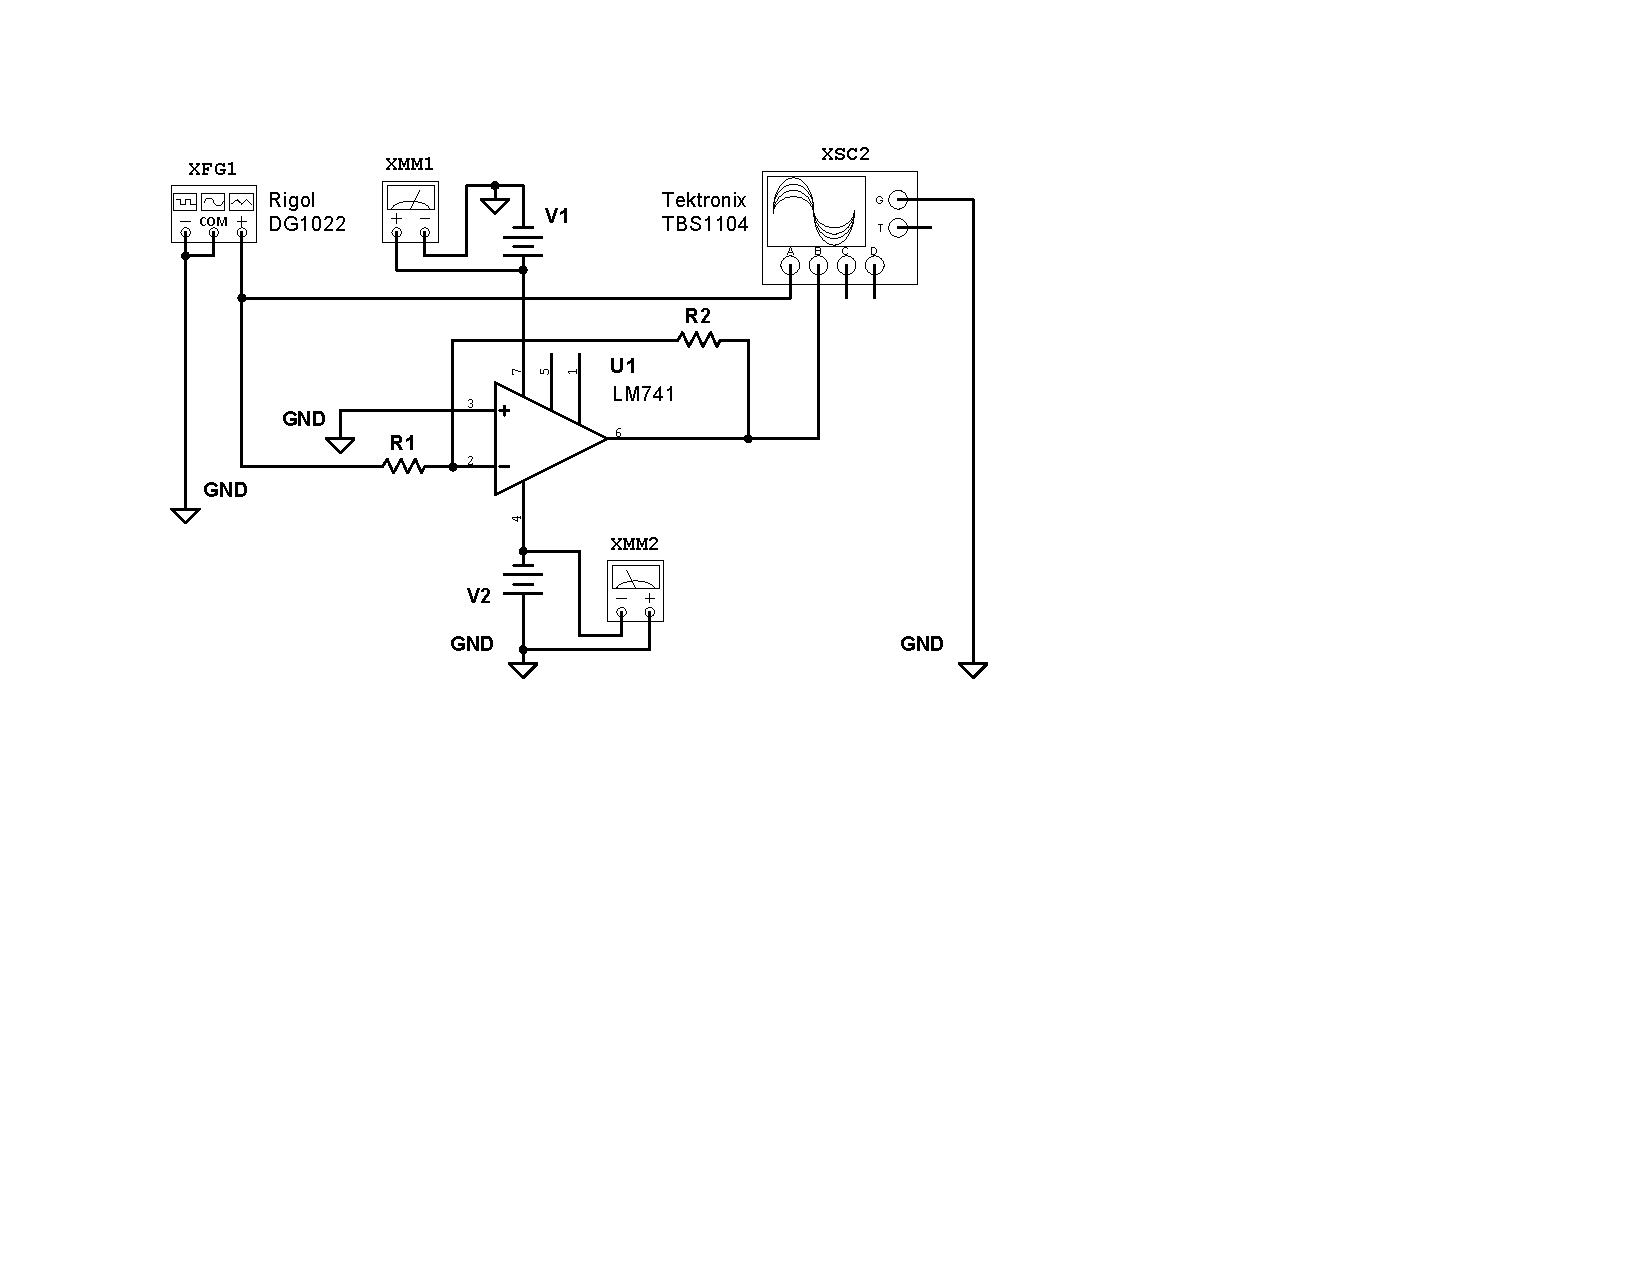
\includegraphics[width=0.38\textwidth]{sch-simulations/output/OPA-closed-loop-inverting.pdf}
\caption{Didascalia}
\label{fig:oscilloscope}
\end {center}
\end{figure}

\subsection{Studio della risposta in frequenza}


%%%%%%%%%%%%%%%%%%%%%%%%%%%%%%%%%%%%%%%%%%
\section{\textbf{Amplificatore reazionato non invertente}} %Matteo
Descrizione

\begin{figure}[H]%[!ht]
\begin {center}
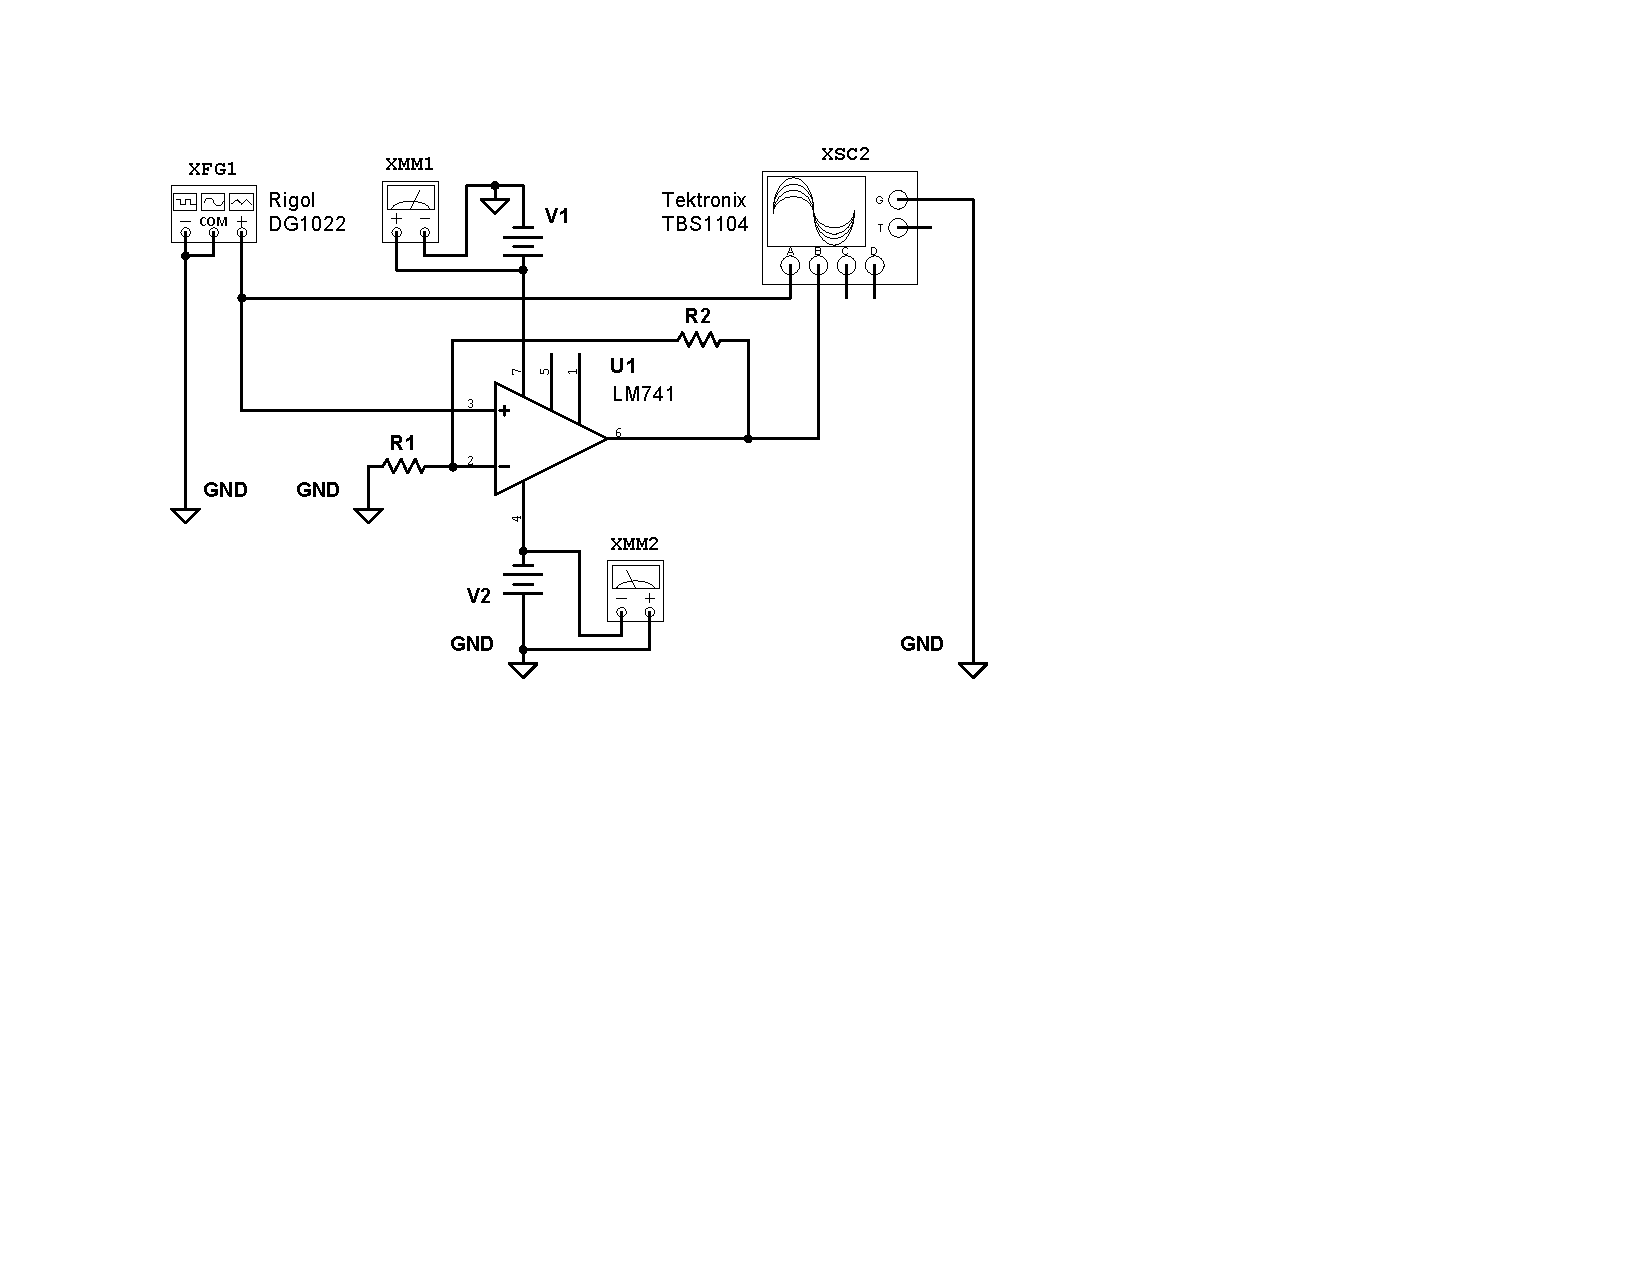
\includegraphics[width=0.38\textwidth]{sch-simulations/output/OPA-closed-loop-non-inverting.pdf}
\caption{Didascalia}
\label{fig:oscilloscope}
\end {center}
\end{figure}

\subsection{Studio della risposta in frequenza}

\subsection{Slew rate}

%%%%%%%%%%%%%%%%%%%%%%%%%%%%%%%%%%%%%%%%%%
\section{Discriminatore ad anello aperto con soglia arbitraria} %Stefano

\begin{figure}[H]%[!ht]
\begin {center}
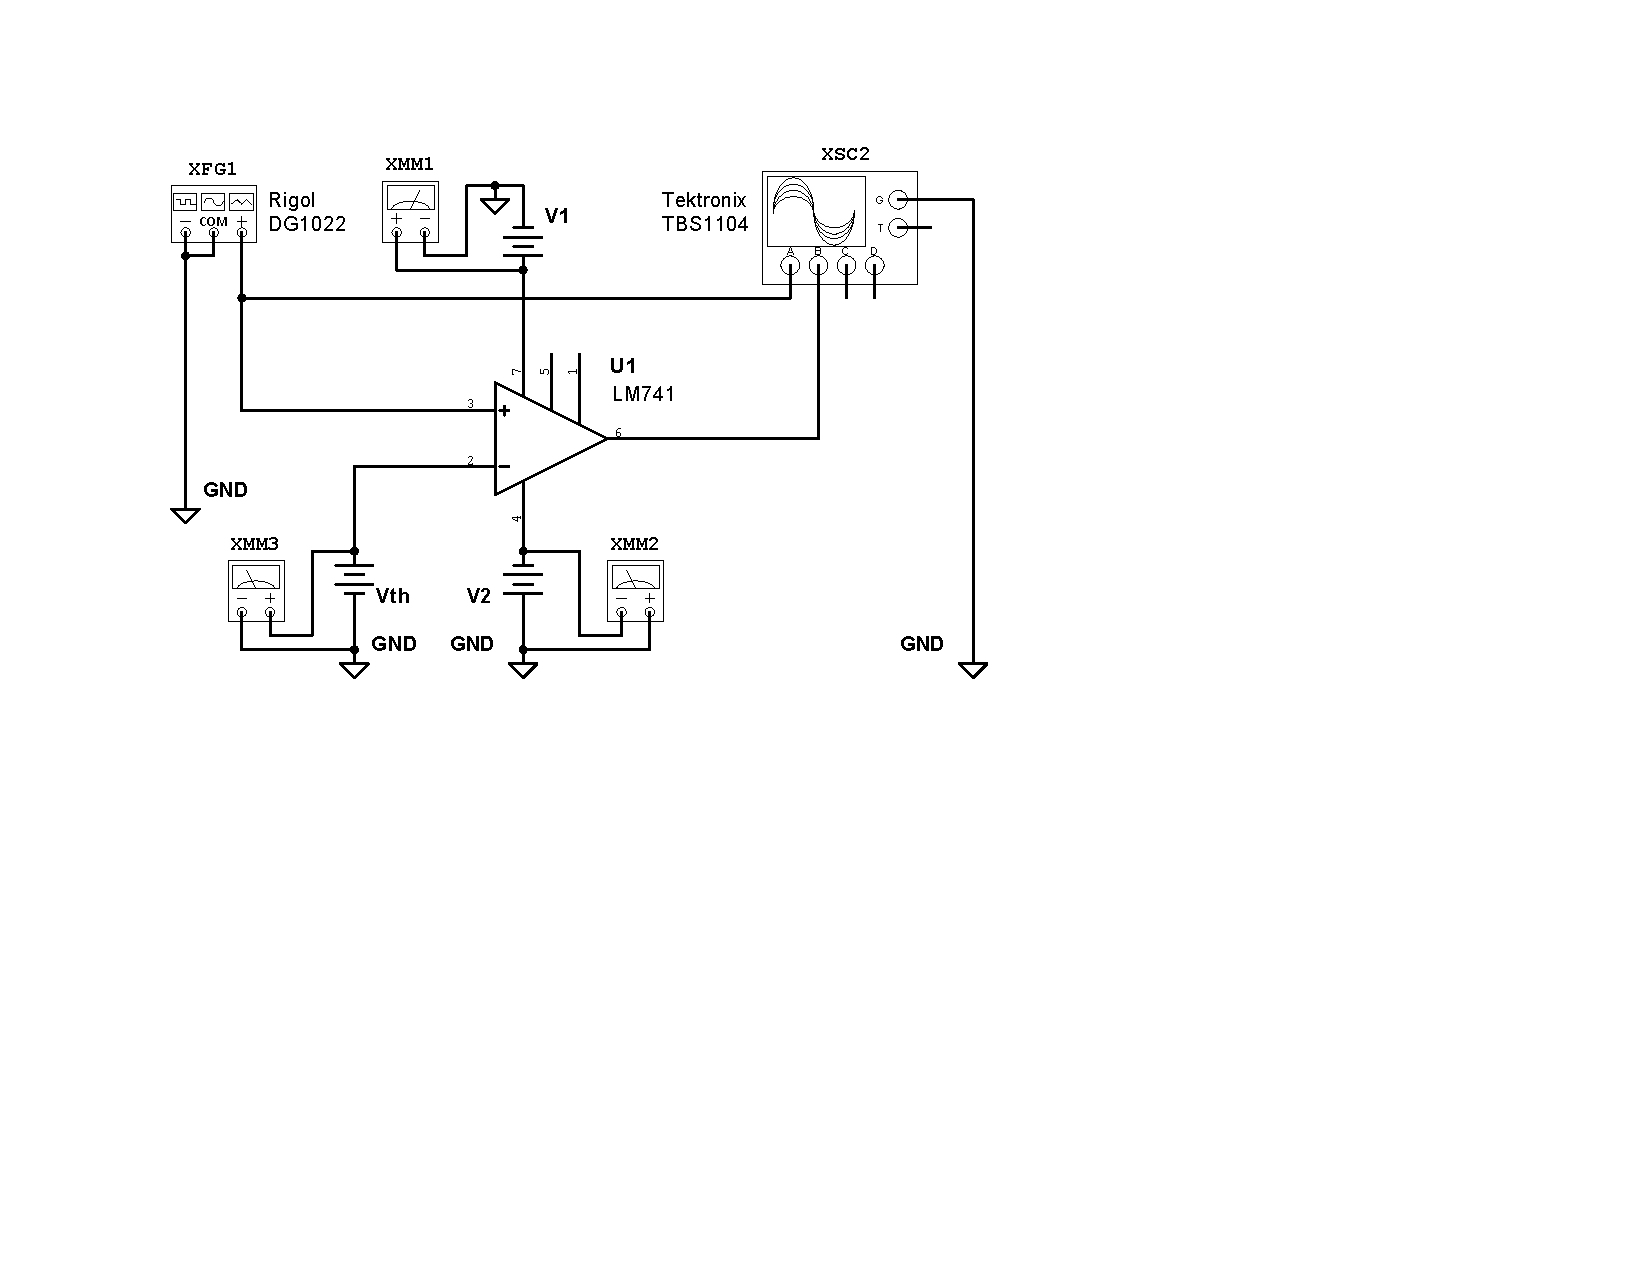
\includegraphics[width=0.38\textwidth]{sch-simulations/output/OPA-biased.pdf}
\caption{Didascalia}
\label{fig:oscilloscope}
\end {center}
\end{figure}

%%%%%%%%%%FINE PRIMO GIORNO%%%%%%%%%%%%%%%
%%%%%%%%%%INIZIO SECONDO GIORNO%%%%%%%%%%%

%%%%%%%%%%%%%%%%%%%%%%%%%%%%%%%%%%%%%%%%%%
\section{Amplificatore logaritmico} %Stefano

\begin{figure}[H]%[!ht]
\begin {center}
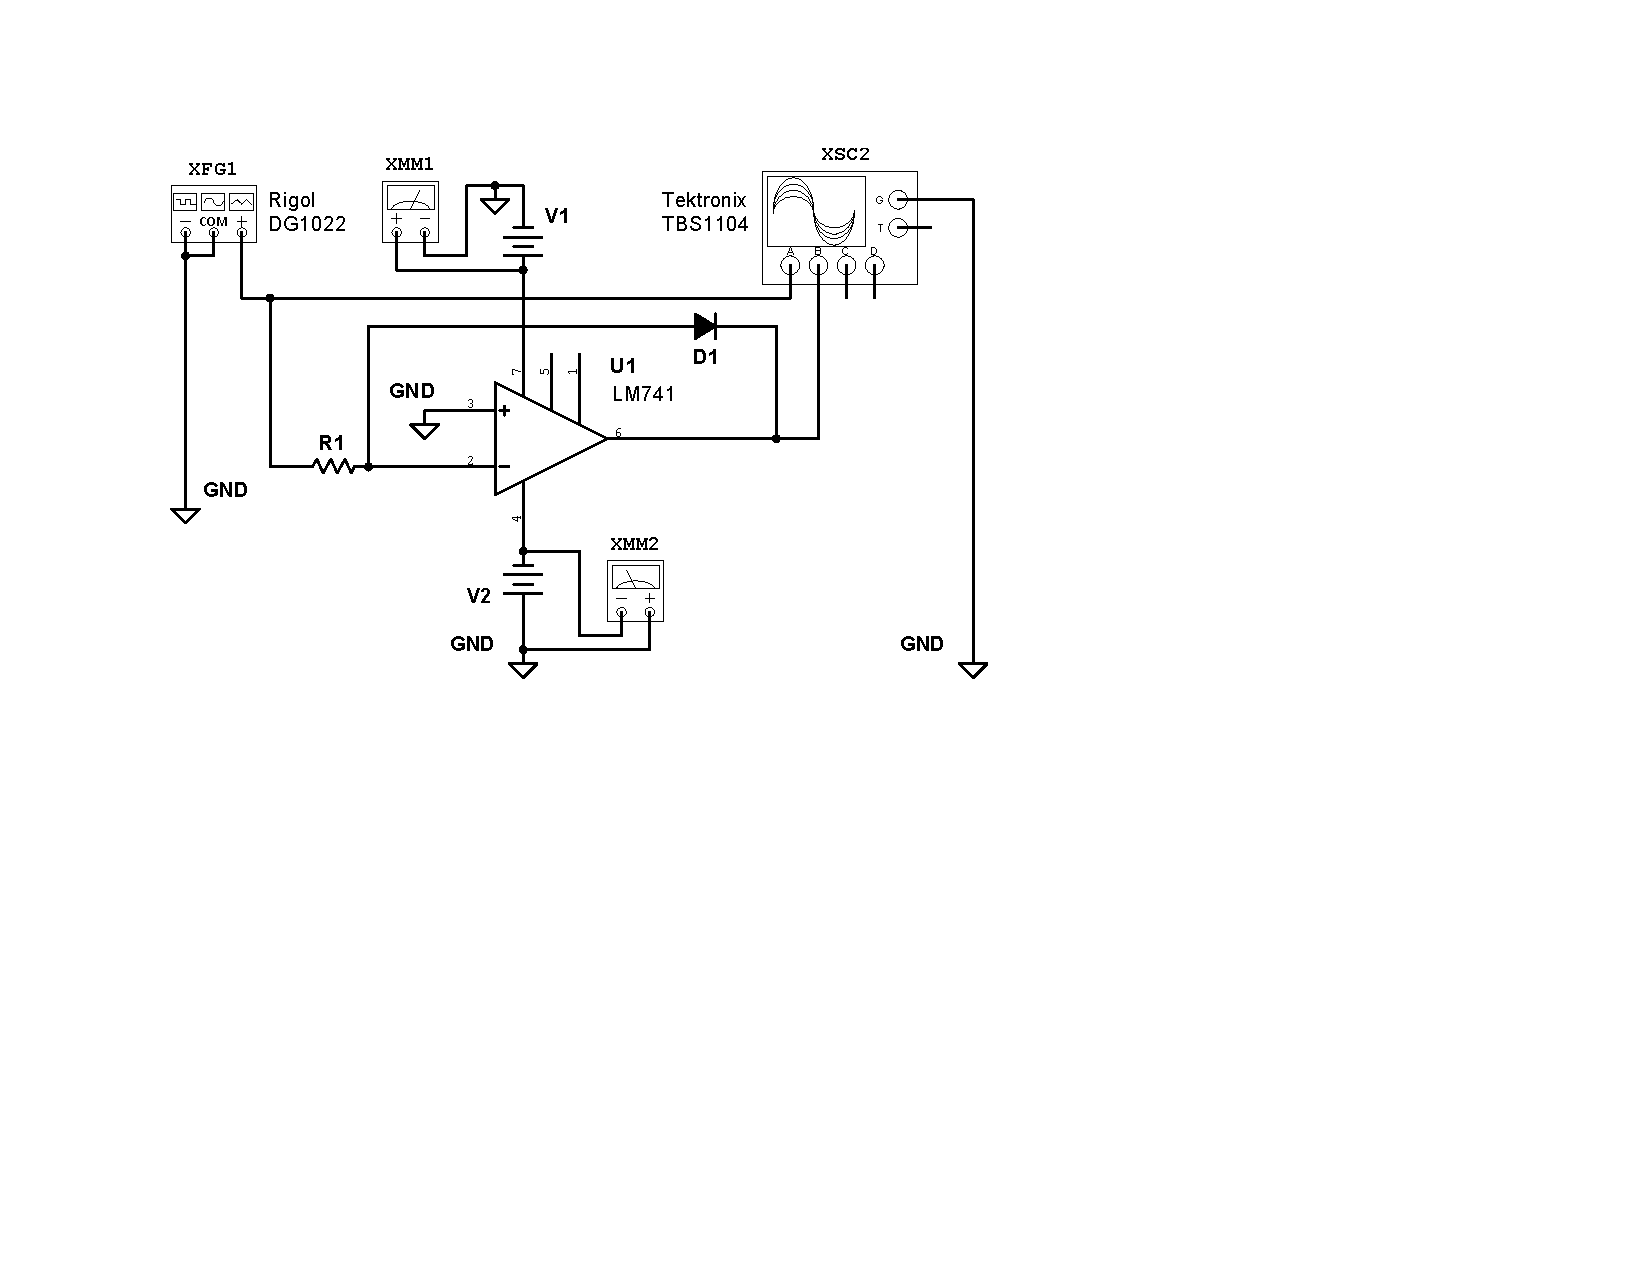
\includegraphics[width=0.38\textwidth]{sch-simulations/output/OPA-log.pdf}
\caption{Didascalia}
\label{fig:oscilloscope}
\end {center}
\end{figure}

%%%%%%%%%%%%%%%%%%%%%%%%%%%%%%%%%%%%%%%%%%
\section{Grafico di risposta}


%%%%%%%%%%%%%%%%%%%%%%%%%%%%%%%%%%%%%%%%%%
\section{Amplificatore integratore} %Matteo

\begin{figure}[H]%[!ht]
\begin {center}
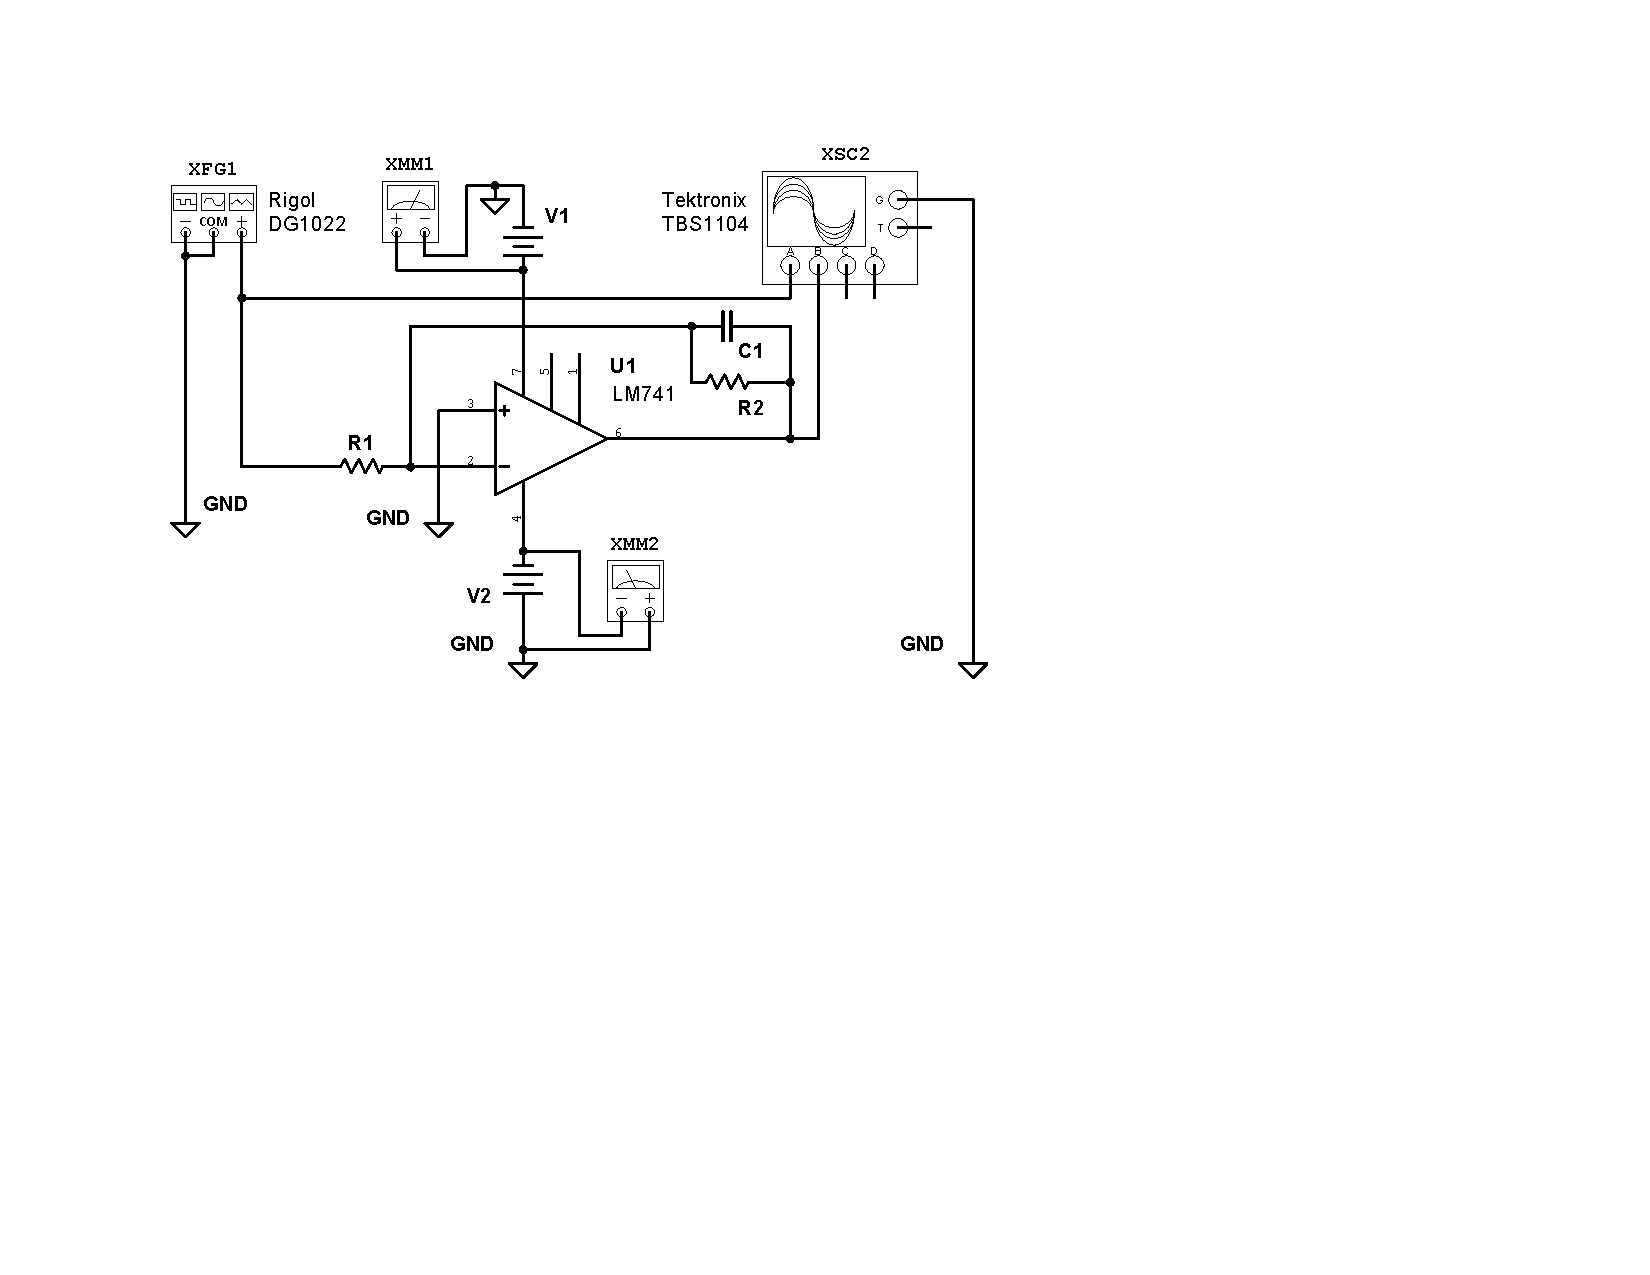
\includegraphics[width=0.38\textwidth]{sch-simulations/output/OPA-integratore.pdf}
\caption{Didascalia}
\label{fig:oscilloscope}
\end {center}
\end{figure}

%%%%%%%%%%%%%%%%%%%%%%%%%%%%%%%%%%%%%%%%%%
\section{Diagramma di Bode}


%%%%%%%%%%%%%%%%%%%%%%%%%%%%%%%%%%%%%%%%%%
\section{Amplificatore derivatore} %Matteo

\begin{figure}[H]%[!ht]
\begin {center}
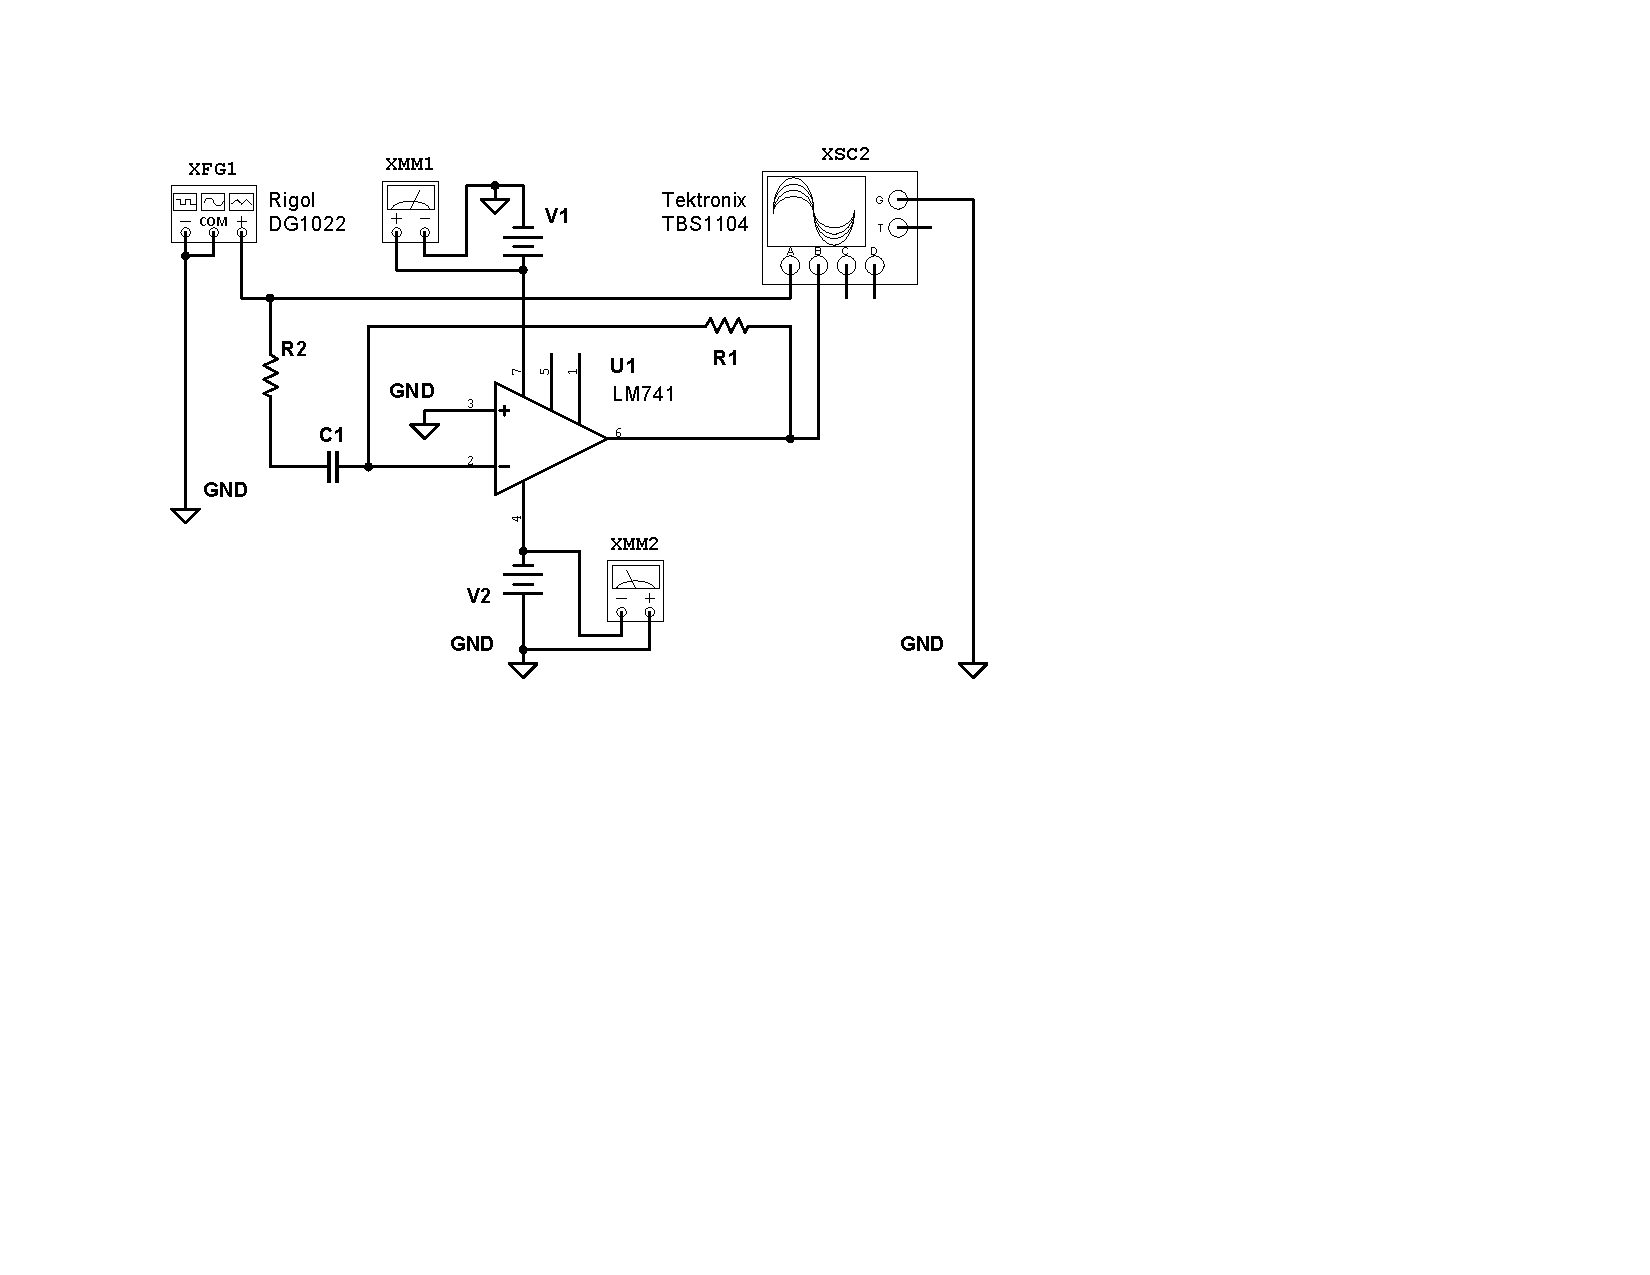
\includegraphics[width=0.38\textwidth]{sch-simulations/output/OPA-deriv.pdf}
\caption{Didascalia}
\label{fig:oscilloscope}
\end {center}
\end{figure}

%%%%%%%%%%FINE SECONDO GIORNO%%%%%%%%%%%%%%%
%%%%%%%%%%INIZIO TERZO GIORNO%%%%%%%%%%%%%%%

%%%%%%%%%%%%%%%%%%%%%%%%%%%%%%%%%%%%%%%%%%
\section{Mixer} %Federico

\begin{figure}[H]%[!ht]
\begin {center}
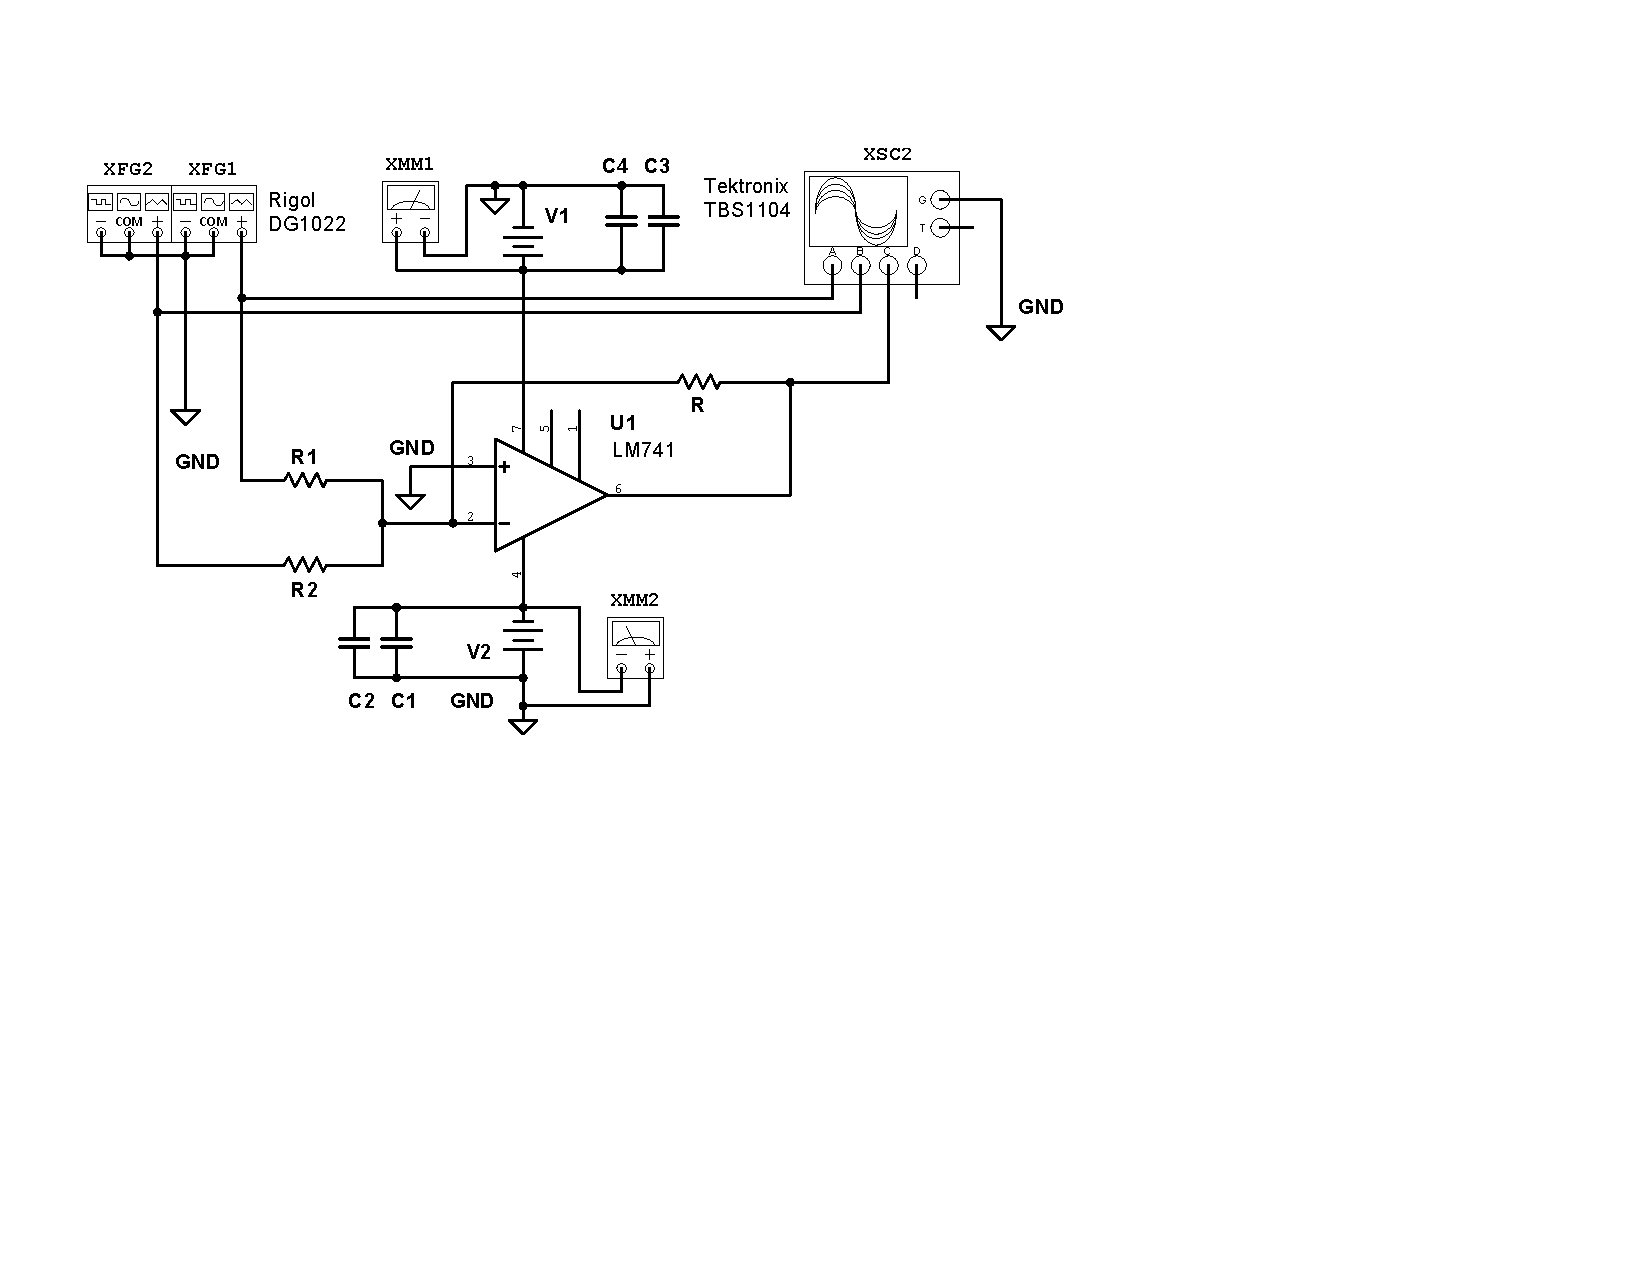
\includegraphics[width=0.38\textwidth]{sch-simulations/output/OPA-mixer.pdf}
\caption{Didascalia}
\label{fig:oscilloscope}
\end {center}
\end{figure}

\subsection{Modulazione e battimenti con ingressi sinusoidali}


%%%%%%%%%%%%%%%%%%%%%%%%%%%%%%%%%%%%%%%%%%
\section{Amplificatore di differenze} %Federico
\begin{figure}[H]%[!ht]
\begin {center}
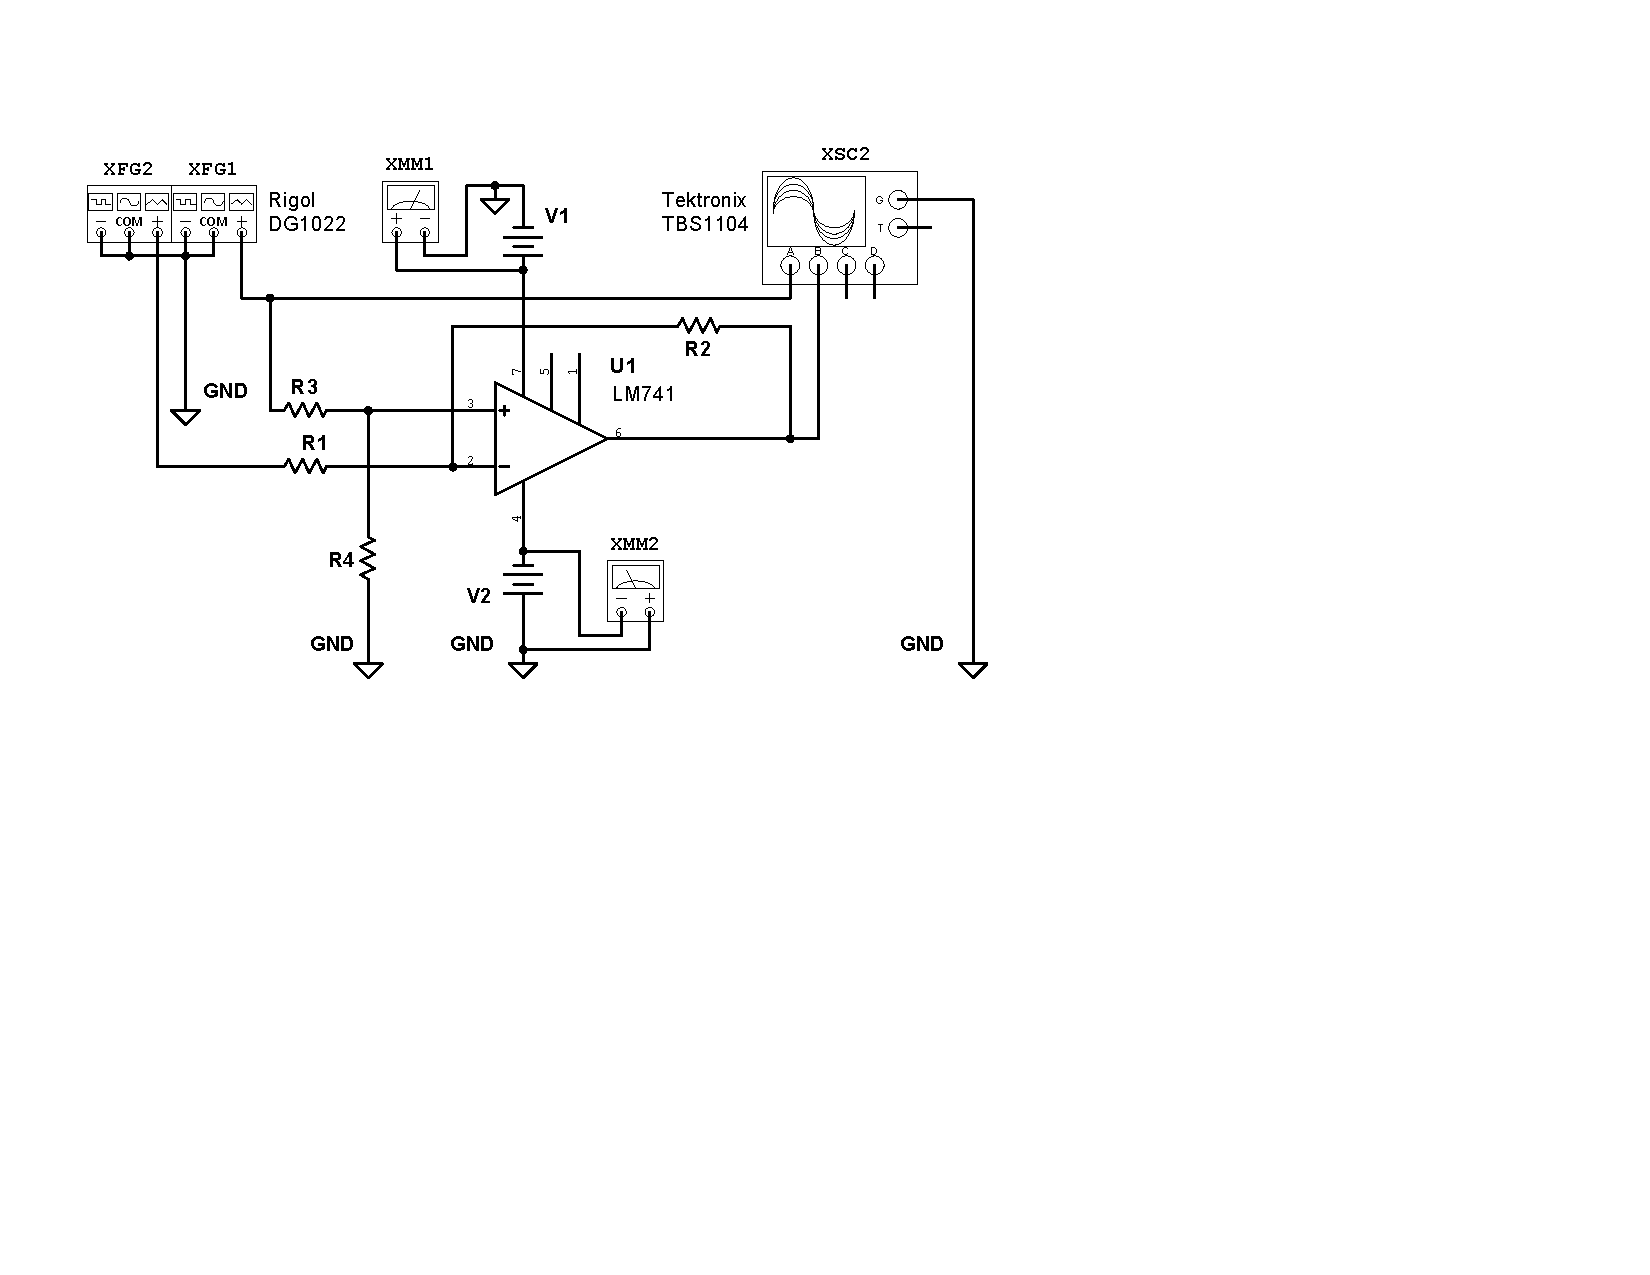
\includegraphics[width=0.38\textwidth]{sch-simulations/output/OPA-difference-amp.pdf}
\caption{Didascalia}
\label{fig:oscilloscope}
\end {center}
\end{figure}

%%%%%%%%%%%%%%%%%%%%%%%%%%%%%%%%%%%%%%%%%%
\section{Trigger di Schmitt} %Federico

\begin{figure}[H]%[!ht]
\begin {center}
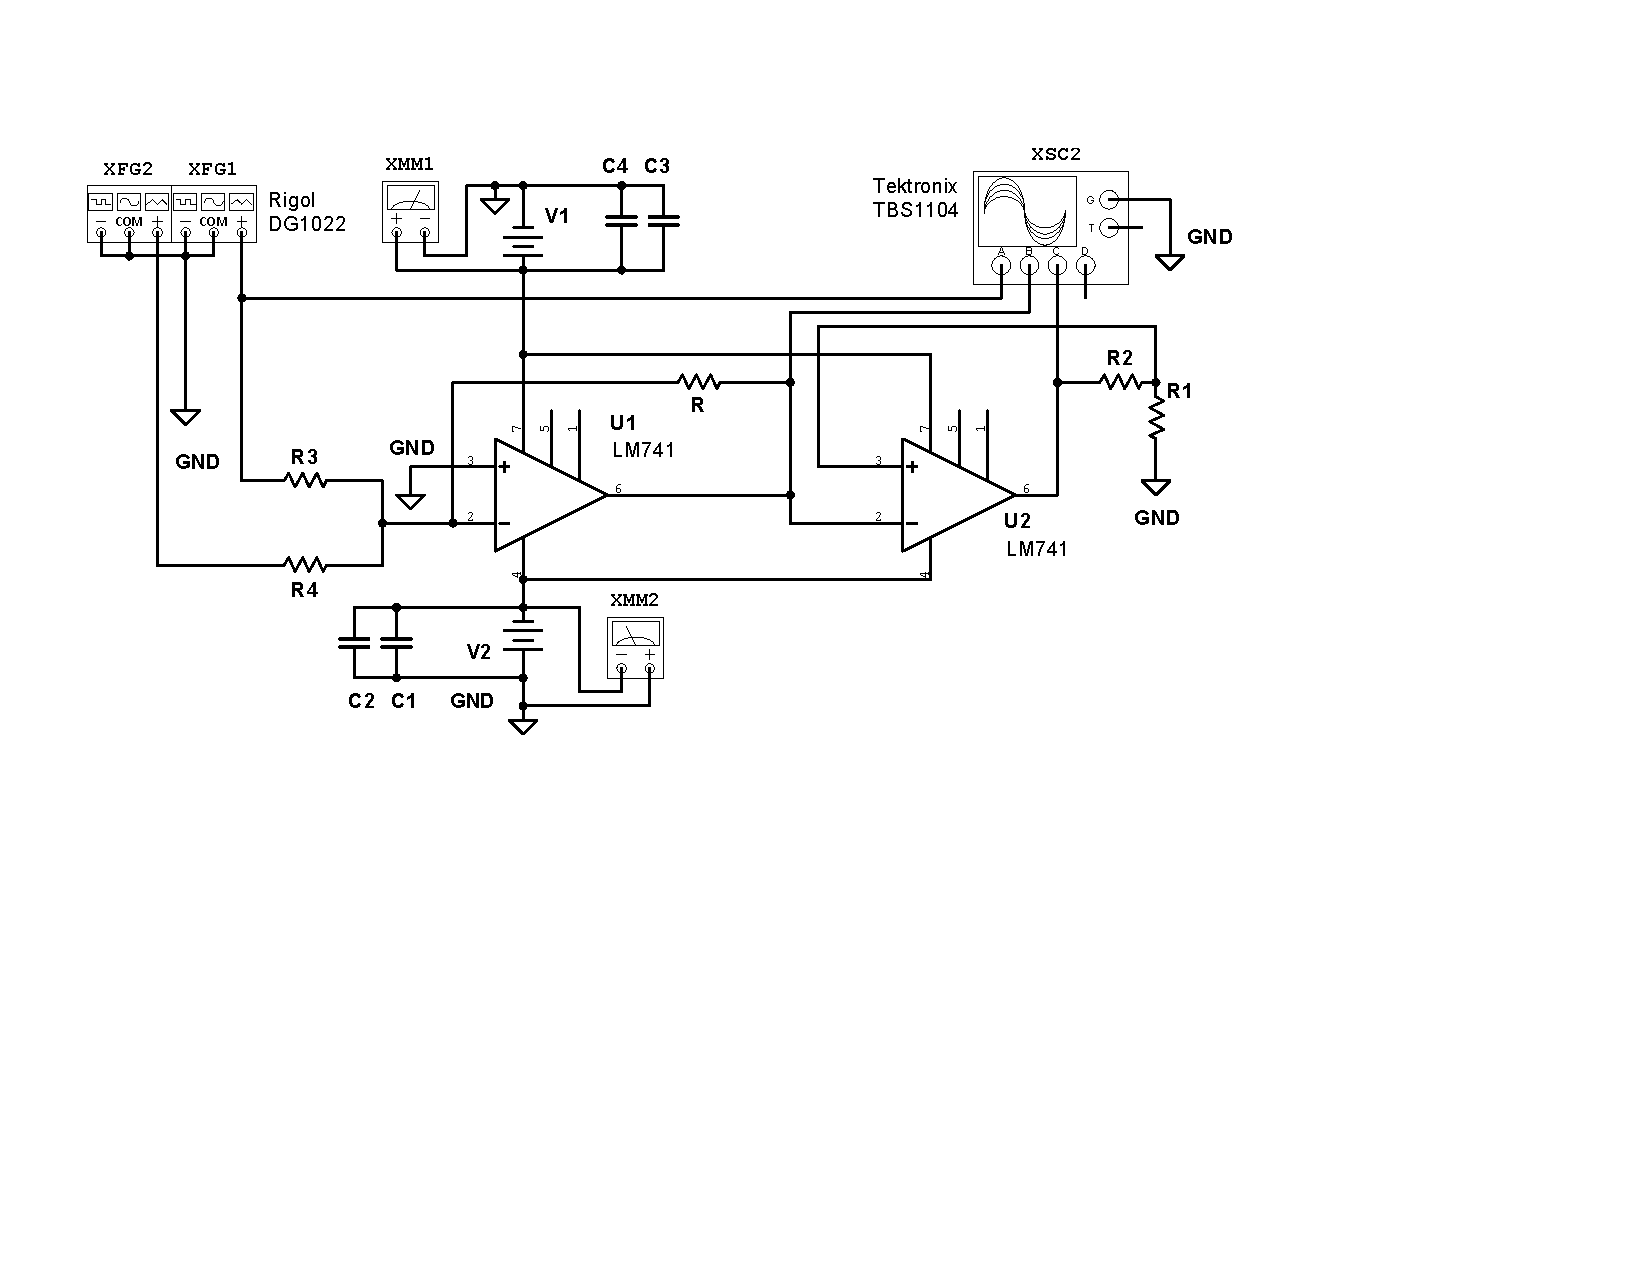
\includegraphics[width=0.48\textwidth]{sch-simulations/output/OPA-mixer-trigger.pdf}
\caption{Didascalia}
\label{fig:oscilloscope}
\end {center}
\end{figure}

\subsection{Ciclo di isteresi al variare della frequenza} %Matteo

%%%%%%%%%%FINE TERZO GIORNO%%%%%%%%%%%%%%%%%%
%%%%%%%%%%INIZIO QUARTO GIORNO%%%%%%%%%%%%%%%

%%%%%%%%%%%%%%%%%%%%%%%%%%%%%%%%%%%%%%%%%%
\section{Silicon photomultiplier} %Valerio

\begin{figure}[H]%[!ht]
\begin {center}
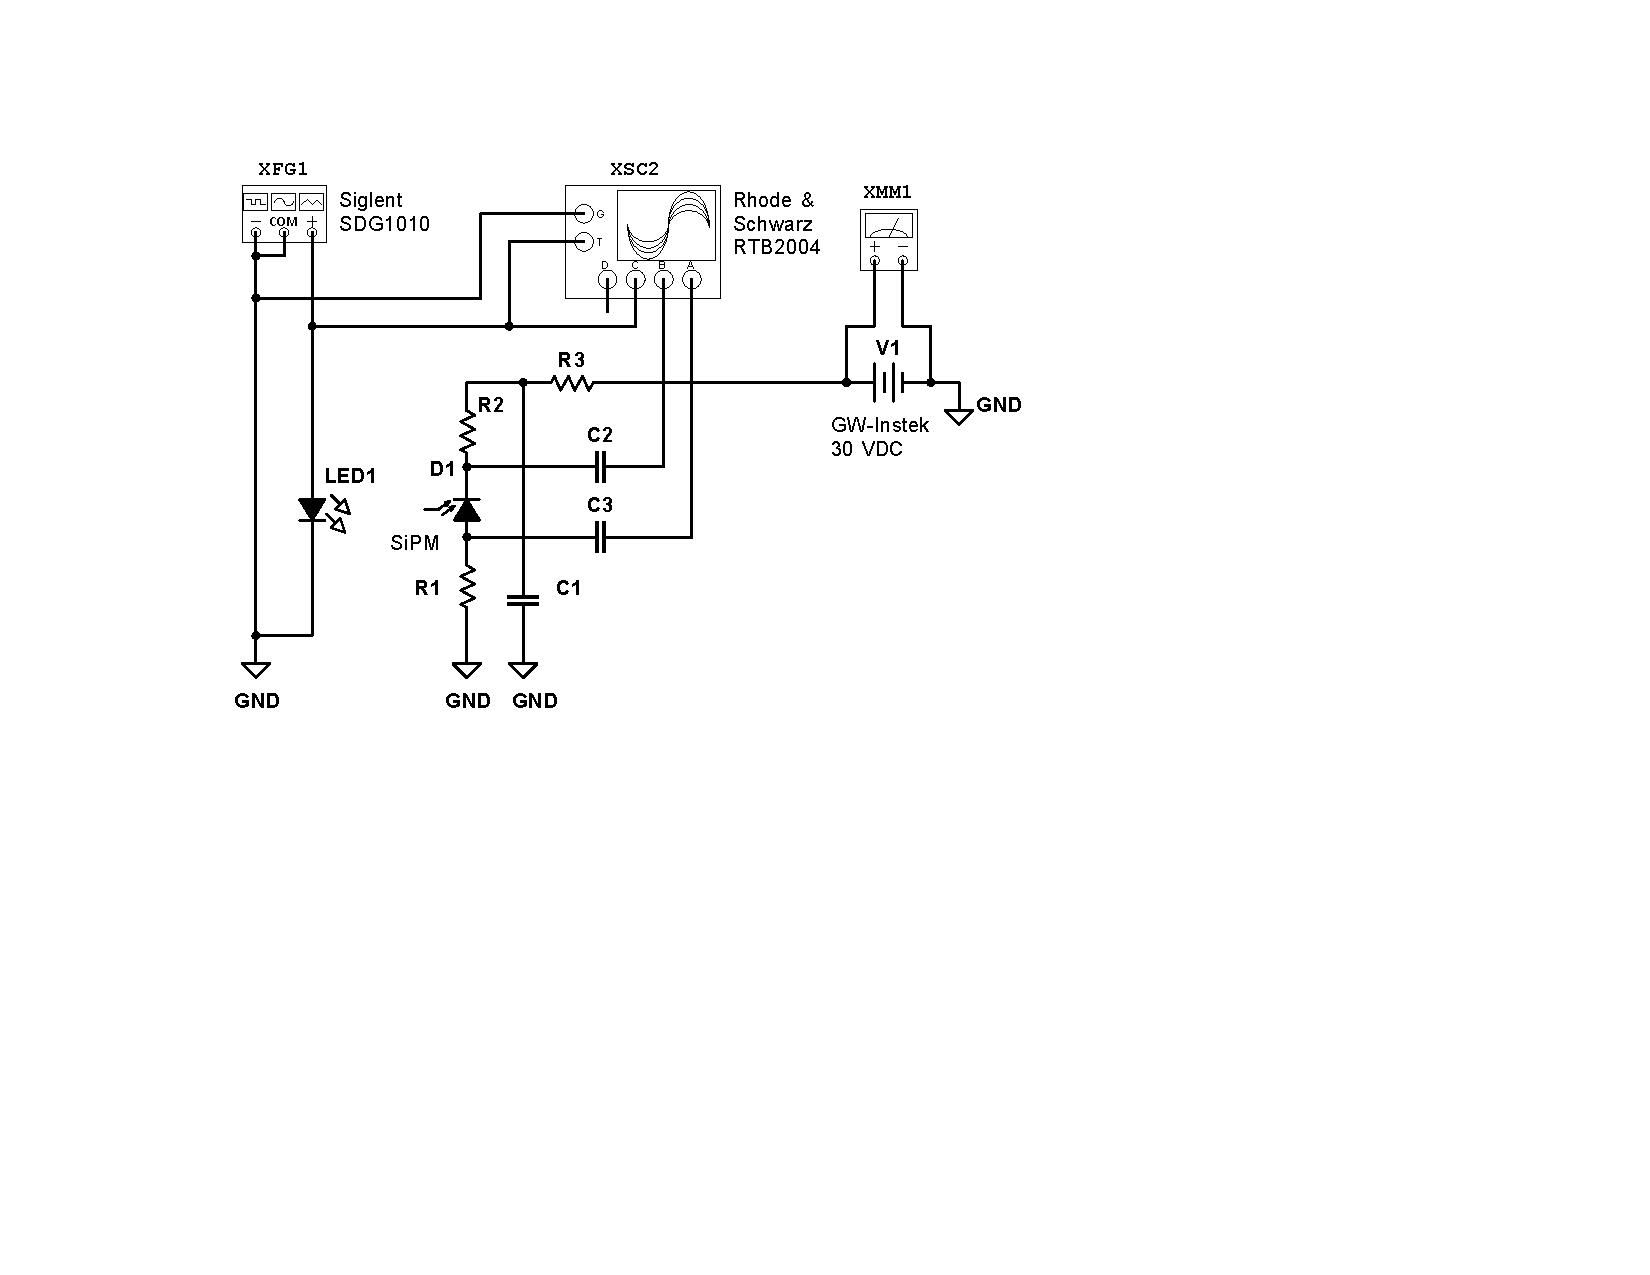
\includegraphics[width=0.46\textwidth]{sch-simulations/output/SiPM.pdf}
\caption{Didascalia}
\label{fig:oscilloscope}
\end {center}
\end{figure}

%%%%%%%%%%%%%%%%%%%%%%%%%%%%%%%%%%%%%%%%%%
\section{Linea di ritardo} %Federico

\section{Silicon photomultiplier} %Valerio

\begin{figure}[H]%[!ht]
\begin {center}
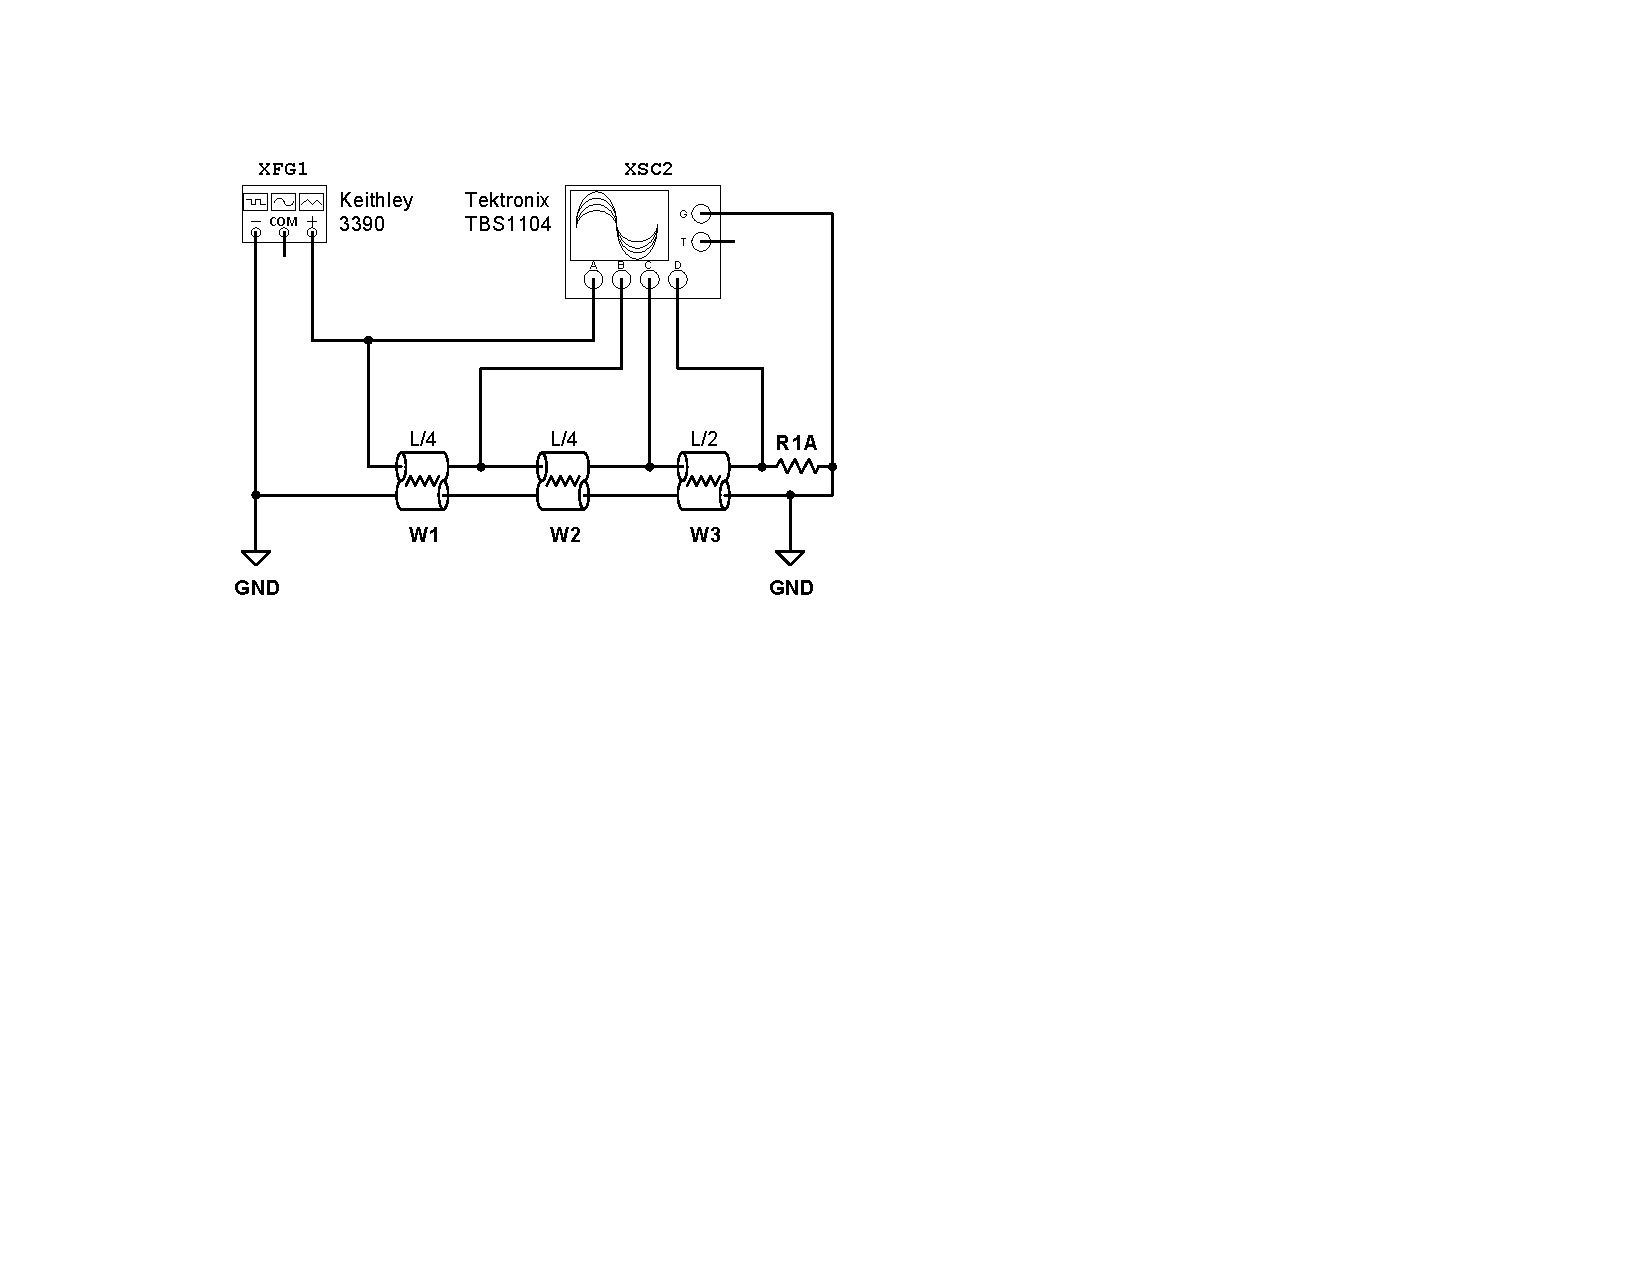
\includegraphics[width=0.38\textwidth]{sch-simulations/output/Transmission line.pdf}
\caption{Didascalia}
\label{fig:oscilloscope}
\end {center}
\end{figure}

\subsection{Tempo di volo impulso singolo}

\subsection{Repetition rate e frequenza di accordatura}

\subsection{Formazione di onde stazionarie}

\subsection{Armoniche 2L}

\subsection{Armoniche L}

%%%%%%%%%%%%%%%%%%%%%%%%%%%%%%%%%%%%%%%%%%
\section{Conclusioni generali} %Valerio e tutti quanti


%%%%%%%%%%%%%%%%%%%%%%%%%%%%%%%%%%%%%%%%%%
\section{Appendice}


%%%%%%%%%%%%%%%%%%%%%%%%%%%%%%%%%%%%%%%%%%
\section{Riferimenti}

\printbibliography


\end{document}


